
\section{開発ソフトの仕様と使用法}
本研究で開発したソフトruby\_noviceは

\begin{enumerate}
\item rubyの標準ライブラリ配布機構であるrubygemsに従っている
\item githubを使って生徒のレポート提出機構を提供している
\item arubaによって生徒自身によるテスト機能を提供している
\end{enumerate}
これらの使い方を理解していただくために,ここで少し詳しく紹介する.

\subsection{ruby\_noviceの振る舞いと意義}
ruby\_noviceは,情報環境であるGitHubを利用しRuby初心者が文法だけでなく,Rubyプログラミングにおける振舞いを身につけるための支援ソフトを開発する.
またRubyプログラミングで重要となるテスト駆動をおこなえる環境を提供している.これにより,学習者自身が出力チェックできるようにしRubyプログラミングにおけるテスト実行に自然と慣れるような学習形態を目指している.

\subsection{ruby\_noviceの仕組み}

\begin{figure}[H]\begin{center}
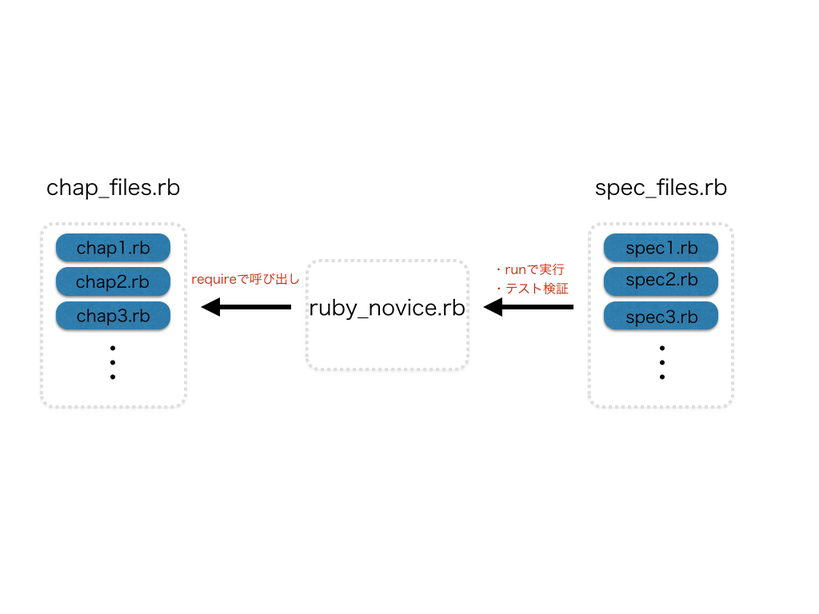
\includegraphics[width=12cm,bb= 0 0 737 553]{../figs/./ruby_novice.001.jpg}
\caption{ruby\_noviceの構造.}

\label{default}\end{center}\end{figure}
ruby\_noviceの構造は,図2のように3つに分かれています.
\begin{itemize}

\item chap\_files.rb (chap1.rb, chap2.rb ...) : Text(たのしいRuby)のコードを書く部分.

\item ruby\_novice.rb : chap\_files.rbを呼び出している.

\item spec\_files.rb : runで外部コマンドを入力して,出力結果 = 期待している値の検証.

\end{itemize}
テストコードが書いているspecファイルを各章ごとに分け,ruby\_novice.rbで呼び出すことにより,章ごとにテストを実行することを可能にした.

以下がruby\_novice.rbのコードの中身である. 
「たのしいRuby」の1章に対応するコードのみを抜粋している.
\begin{lstlisting}[style=customRuby,basicstyle={\scriptsize\ttfamily}]
 #ruby_novice.rb
 
 $LOAD_PATH.unshift File.expand_path("../../lib/#{ENV['RUBYNOVICE_NAME']}", __FILE__)
 begin
   require "chap_files"
 rescue LoadError
   p "Load Error of ex_files in rubynovice.rb."
   p File.expand_path("../../lib/#{ENV['RUBYNOVICE_NAME']}", __FILE__)
   exit
 end
 
 require "ruby_novice/version"
 require 'thor'
 #require "code"                                                                                  
 
 module RubyNovice
   # Your code goes here...                                                                       
 
   class CLI < Thor
 #    class_option :help, type: :boolean, aliases: '-h', desc: 'help.'                            
 #    class_option :debug, type: :boolean, aliases: '-d', desc: 'debug mode'                      
 
 =begin                                                                                           
     desc 'hello', 'print hello'                     
     def hello                                                                                    
       my_hello                                                                                   
     end                                                                                          
 =end
 
     desc 'my_helloruby', 'print helloruby'
     def my_helloruby
       helloruby
     end
 
     desc 'my_puts_and_p', 'print puts_and_p'
     def my_puts_and_p
       puts_and_p
     end
 
     desc 'my_kiritsubo', 'print kiritsubo'
     def my_kiritsubo
       kiritsubo
     end
 
     desc 'my_area_volume', 'print area_volume'
     def my_area_volume
       area_volume
     end
 
     desc 'my_comment_sample', 'print comment_sample'
     def my_comment_sample
       comment_sample
     end
 
     desc 'my_greater_smaller', 'print greater_smaller'
     def my_greater_smaller
       greater_smaller
     end
 
     desc 'my_greater_smaller_else', 'print greater_smaller_else'
     def my_greater_smaller_else
       greater_smaller_else
     end
 
     desc 'version', 'version'
     def version
       puts RubyNovice::VERSION
     end
 
     private
 
     def output_error_if_debug_mode(e)
       return unless options[:debug]
       STDERR.puts(e.message)
       STDERR.puts(e.backtrace)
     end
   end
 end
\end{lstlisting}

以下はchap1\_spec.rb のコードの中身である. 
Text(たのしいRuby)の1章に対応するspec codeを書き出している.

\begin{lstlisting}[style=customRuby,basicstyle={\scriptsize\ttfamily}]
 #spec_chap1.rb
 require 'spec_helper'
 
 RSpec.describe 'ruby_novie command', type: :aruba do
   context 'version option', type: :version do
     before(:each) { run('ruby_novice v') }
     it { expect(last_command_started).to be_successfully_executed }
     it { expect(last_command_started).to have_output("0.1.0") }
   end
 
   context 'help option', type: :help do
     expected = `bundle exec exe/ruby_novice help`
     before(:each) { run('ruby_novice help') }
     it { expect(last_command_started).to be_successfully_executed }
 #   it { expect(last_command_started).to have_output(expected) }               
   end
 
 =begin                                                                          
   context 'print hello', type: :hello do                                        
     before(:each) { run('ruby_novice hello') }                                  
     expected = "Hello."                                                         
     it { expect(last_command_started).to be_successfully_executed }             
     it { expect(last_command_started).to have_output(expected) }    
   end                                                                           
 =end 
 
   context 'helloruby', type: :helloruby do
     before(:each) { run('ruby_novice my_helloruby') }
     expected = "Hello, Ruby."
     it { expect(last_command_started).to be_successfully_executed }
     it { expect(last_command_started).to have_output(expected) }
   end
 
   context 'puts_and_p', type: :puts_and_p do
     before(:each) { run('ruby_novice my_puts_and_p') }
     expected = "Hello,\n\tRuby.\n\"Hello,\n\tRuby.\""
 
     it { expect(last_command_started).to be_successfully_executed }
     it { expect(last_command_started).to have_output(expected) }
   end
 
   context 'kiritsubo', type: :kiritsubo do
     before(:each) { run('ruby_novice my_kiritsubo') }
     expected = "いづれの御時にか女御更衣あまたさぶらいたまいけるなかに\nいとや\\
 むごとなき際にはあらぬがすぐれて時めきたまふありけり"
 
     it { expect(last_command_started).to be_successfully_executed }
     it { expect(last_command_started).to have_output(expected) }
   end
 
   context 'area_volume', type: :area_volume do
     before(:each) { run('ruby_novice my_area_volume') }
     expected = "表面積=2200\n体積=6000"
 
     it { expect(last_command_started).to be_successfully_executed }
     it { expect(last_command_started).to have_output(expected) }
   end
 
   context 'greater_smaller', type: :greater_smaller do
     before(:each) { run('ruby_novice my_greater_smaller') }
     expected = "greater"
 
     it { expect(last_command_started).to be_successfully_executed }
     it { expect(last_command_started).to have_output(expected) }
   end
 
 
   context 'greater_smaller_else', type: :greater_smaller_else do
     before(:each) { run('ruby_novice my_greater_smaller_else') }
     expected = "greater"
 
     it { expect(last_command_started).to be_successfully_executed }
     it { expect(last_command_started).to have_output(expected) }
   end
 end
\end{lstlisting}

chap1\_spec.rbなどが呼び出すspec\_helper.rbは以下の通りである.\$LOAD\_PATHにgemの標準構造の
場合に配置されるlibを入れている.また,その後はsupport directoryであるが,RUBYのversionが
古い場合にも対応するように設定している.

\begin{lstlisting}[style=customRuby,basicstyle={\scriptsize\ttfamily}]
#spec_helper.rb
$LOAD_PATH.unshift File.expand_path('../../lib', __FILE__)
require 'ruby_novice'
#require 'aruba/rspec'
$LOAD_PATH.unshift File.expand_path('../../lib', __FILE__)

if RUBY_VERSION < '1.9.3'
  ::Dir.glob(::File.expand_path('../support/*.rb', __FILE__)).each { |f| require File.join(File.dirname(f), File.basename(f, '.rb')) }
  ::Dir.glob(::File.expand_path('../support/**/*.rb', __FILE__)).each { |f| require File.join(File.dirname(f), File.basename(f, '.rb')) }
else
  ::Dir.glob(::File.expand_path('../support/*.rb', __FILE__)).each { |f| require_relative f }
  ::Dir.glob(::File.expand_path('../support/**/*.rb', __FILE__)).each { |f| require_relative f }
end
\end{lstlisting}
\subsection{ruby\_noviceの現状}

現状は,「たのしいRuby」の第1章〜第7章までのテストコードを書き実装できる.
各章の概要は,以下の通りである.

\begin{itemize}
\item 第1章 (list1.1 〜 1.7):  putsメソッドやpメソッド.
\item 第3章 (list3.1 〜 3.11): ファイルの読み込み.
\item 第4章 (list4.1):        ローカル変数とグローバル変数.
\item 第5章 (list5.1 〜 5.5):  条件判断.(if, unlessなど)
\item 第6章 (list6.1 〜 6.13): 繰り返し.(for,times,whileなど)
\item 第7章 (list7.1 〜 7.4):  メソッド.
\end{itemize}
\subsubsection{注意}

「たのしいRuby」の課題では,問題番号以外に,コードに対応する適当なプログラム名が付されている.
しかし,Rub言語の予約語(for,whileなど)はコード中で使えないため,
以下の問題は名前を変更して"1"をつけている.

\begin{itemize}
\item list5.3:  unless.rb → unless1.rbに変更.
\item list5.4:  case.rb → case1.rbに変更.
\item list6.4:  for.rb → for1.rbに変更.
\item list6.6:  while.rb → while11.rbに変更.
\item list6.9:  until.rb → until1.rbに変更.
\item list7.4:  myloop.rb → myloop1.rbに変更.
\end{itemize}
\subsection{ruby\_noviceの作業の流れ}
\begin{figure}[H]\begin{center}
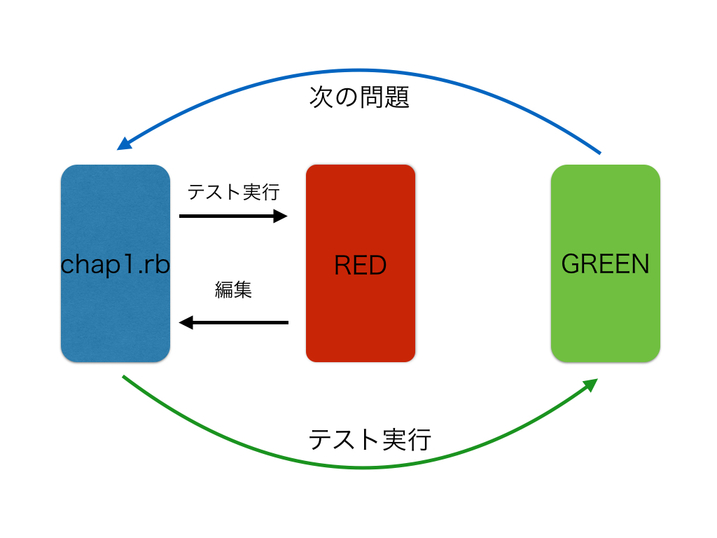
\includegraphics[width=12cm,bb= 0 0 737 553]{../figs/./ruby_novice.003.jpg}
\caption{学習の流れ.}
\label{default}\end{center}\end{figure}

図3のようにRuby学習者はRed, Greenという作業サイクルを繰り返してプログラミングを進めていく.

\begin{enumerate}
\item 作成したいプログラムの仕様を明確にする.
\item Red (テストに失敗)
\item Green(Redの状態ならば,編集しテストを成功させるコードを書く)
\item Greenになると次の問題に進む.
\end{enumerate}
Red,Greenという言葉は,TDDで多用されるテスティングフレームワークの多くがテスト失敗を赤色表示で,テスト成功を緑色表示で通知することに由来している.
図4がテストにパスした時の出力結果で,図5がテストに失敗した時の出力結果である.色を見るだけでテストをパスしているか失敗しているか一目瞭然である.

\begin{figure}[H]\begin{center}
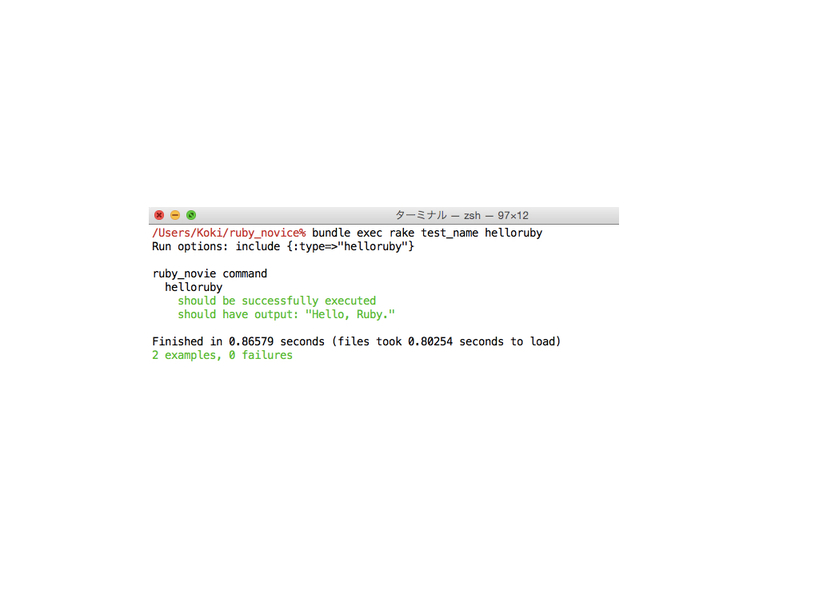
\includegraphics[width=12cm,bb= 0 0 737 553]{../figs/./ruby_novice.004.jpg}
\caption{Greenの出力結果.}
\label{default}\end{center}\end{figure}
\begin{figure}[H]\begin{center}
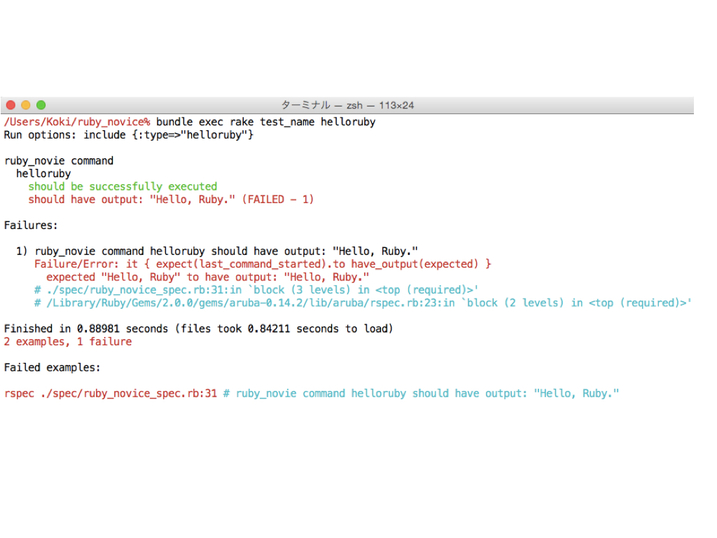
\includegraphics[width=12cm,bb= 0 0 737 653]{../figs/./ruby_novice.005.jpg}
\caption{Redの出力結果.}
\label{default}\end{center}\end{figure}
\subsection{ruby\_noviceの使用法}

1. 自分の好きな名前(koki)をつけたディレクトリを作成する.

2. ./lib/koki/chap\_files.rbを準備する.

3. chap\_files.rbの中にrequire "chap1"と書く.

4. chap1.rbというファイルを作り,そのファイルにたのしいRuby1章のlist(1.1~1.7)のコードを書いていく.

5. rspecで,個人ごとの検査を実行する場合,環境変数RUBYNOVICE\_NAMEに各自で決めたディレクトリ名(koki)を入れる.

\begin{itemize}
\item (csh,tcsh)setenv RUBYNOVICE\_NAME koki
\item (bash,zsh)export RUBYNOVICE\_NAME=koki
\end{itemize}

コード例
\begin{lstlisting}[style=customRuby,basicstyle={\scriptsize\ttfamily}]
  #/Users/Koki/ruby_novice% cat lib/koki/chap_files.rb
  
  require "chap1"
  #require "chap3" 
  #require "chap4"
  #require "chap5"
  #require "chap6"
  #require "chap7"

  (注) # はコメントアウト.
\end{lstlisting}

コード例 (たのしいRuby第1章)

\begin{lstlisting}[style=customRuby,basicstyle={\scriptsize\ttfamily}]
 #/Users/Koki/ruby_novice% cat lib/koki/chap1.rb
 
 def helloruby     
   print("Hello, Ruby.\n")
 end
 
 def puts_and_p
   puts "Hello,\n\tRuby."
   p "Hello,\n\tRuby."
 end
 
 def kiritsubo
   print "いづれの御時にか女御更衣あまたさぶらいたまいけるなかに\n"
   print "いとやむごとなき際にはあらぬがすぐれて時めきたまふありけり\n"
 end
 
 def area_volume
   x = 10
   y = 20
   z = 30
   area = (x*y + y*z + z*x) * 2
   volume = x * y * z
   print "表面積=", area, "\n"
   print "体積=", volume, "\n"
 end
 
 def comment_sample
 =begin                                                                          
   「たのしいRuby 第5版」サンプル                                               
    コメントの使い方の例                                                         
   2006/06/16 作成                                                              
    2006/07/01 一部コメントを追加                                                
    2015/10/01 第5版用に更新                                                    
 =end
 
   x = 10 # 縦                                                                   
   y = 20 # 縦                                                                   
   z = 30 # 高さ                                                                 
   # 表面積と体積を計算する                                                      
   area = (x*y + y*z + z*x) * 2
   volume = x * y * z
   # 出力する                                                                    
   print "表面積=", area, "\n"
   print "体積=", volume, "\n"
 end
 
 def greater_smaller
   a = 20
   if a >= 10 then
     print "greater\n"
   end
   if a <= 9 then
     print "smaller\n"
   end
 end
 
 def greater_smaller_else
   a = 20
   if a >= 10
     print "greater\n"
   else
     print "smaller\n"
   end
 end
\end{lstlisting}
\subsubsection{Tagの表示の仕方}

1. grep type spec/ruby\_novice\_spec.rb  で全てのcontextとtypeを表示.
typeは各章の各問題名に相当する.各問題ごとにテストする時の便宜となる.

\begin{lstlisting}[style=customRuby,basicstyle={\scriptsize\ttfamily}]
  context 'version option', type: :version do
  context 'help option', type: :help do
  context 'print hello', type: :hello do
  context 'helloruby', type: :helloruby do
  context 'puts_and_p', type: :puts_and_p do
  context 'kiritsubo', type: :kiritsubo do
  context 'area_volume', type: :area_volume do
  context 'comment_sample', type: :comment_sample do
  context 'greater_smaller', type: :greater_smaller do
  context 'greater_smaller_else', type: :greater_smaller_else do
  context 'print_argv', type: :print_argv do
  context 'happy_birth', type: :happy_birth do
  context 'arg_arith', type: :arg_arith do
  context 'read_text', type: :read_text do
  context 'read_text_simple', type: :read_text_simple do
  context 'read_text_oneline', type: :read_text_oneline do
  context 'read_line', type: :read_line do
  context 'simple_grep', type: :simple_grep do
  context 'hello_ruby2', type: :hello_ruby2 do
  context 'use_grep', type: :use_grep do
  context 'scopetest', type: :scopetest do
  context 'ad2heisei', type: :ad2heisei do
  context 'if_elsif', type: :if_elsif do
  context 'unless1', type: :unless1 do
  context 'case1', type: :case1 do
  context 'case_class', type: :case_class do
  context 'times', type: :times do
  context 'times2', type: :times2 do
  context 'times3', type: :times3 do
  context 'for1', type: :for1 do
  context 'for_names', type: :for_names do
  context 'while1', type: :while1 do
  context 'while2', type: :while2 do
  context 'while3', type: :while3 do
  context 'until1', type: :until1 do
  context 'while_not', type: :while_not do
  context 'each_names', type: :each_names do
  context 'each', type: :each do
  context 'break_next', type: :break_next do
  context 'times_with_param', type: :times_with_param do
  context 'hello_with_name', type: :hello_with_name do
  context 'hello_with_default', type: :hello_with_default do
  context 'myloop1', type: :myloop1 do
\end{lstlisting}
\subsection{全章のテストの仕方}

1. bundle exec rspec

すべての章のテストを一括して実行できる.

\subsection{各章ごとのテストの仕方}

例: 1章(chap1)のテストをしたい時.

1. bundle exec rspec spec/chap1\_spec.rb

2. bundle exec rake chap 1

実行例

\begin{lstlisting}[style=customRuby,basicstyle={\scriptsize\ttfamily}]
 /Users/Koki/ruby_novice% bundle exec rake chap 1   
 
 ruby_novie command
   version option
     should be successfully executed
     should have output: "0.1.0"
   help option
     should be successfully executed
   helloruby
     should be successfully executed
     should have output: "Hello, Ruby."
   puts_and_p
     should be successfully executed
     should have output: "Hello,\n\tRuby.\n\"Hello,\n\tRuby.\""
   kiritsubo
     should be successfully executed
     should have output: "いづれの御時にか女御更衣あまたさぶらいたまいけるなかに\nいとやむごとなき際にはあらぬがすぐれて時めきたまふありけり"
   area_volume
     should be successfully executed
     should have output: "表面積=2200\n体積=6000"
   comment_sample
     should be successfully executed
     should have output: "表面積=2200\n体積=6000"
   greater_smaller
     should be successfully executed
     should have output: "greater"
   greater_smaller_else
     should be successfully executed
     should have output: "greater"
		 
 Finished in 7.61 seconds (files took 1.03 seconds to load)
 17 examples, 0 failures
\end{lstlisting}
\subsubsection{各問題ごとのテストの仕方}
例: 各問題(helloruby)ごとにテストをしたい時.

1. bundle exec rspec --tag type:helloruby spec/ruby\_novice\_spec.rb  (hellorubyは問題名)

2. bundle exec rake test\_name helloruby

実行例
\begin{lstlisting}[style=customRuby,basicstyle={\scriptsize\ttfamily}]
/Users/Koki/ruby_novice% bundle exec rake test_name helloruby
Run options: include {:type=>"helloruby"}

ruby_novie command
  helloruby
    should be successfully executed
    should have output: "Hello, Ruby."
		 
Finished in 0.87128 seconds (files took 0.81684 seconds to load)
2 examples, 0 failures
\end{lstlisting}

問題名は,上記のgrep type spec/ruby\_novice\_spec.rbで調べることができる.
typeが各問題の名前になる.またtextの問題名(例えばputs\_and\_p.rb)が,そのまま使えるのでテストも簡単にでき,問題名で中身のコードの内容も把握できる.

\subsubsection{各問題ごとの実行結果の出力}
例として, 下記に print("Hello, Ruby.") のコードを入力する問題であるhelloruby.rbの実行結果の出力を示す.

1. bundle exec exe/ruby\_novice my\_helloruby

2. bundle exec rake/output helloruby

実行例
\begin{lstlisting}[style=customRuby,basicstyle={\scriptsize\ttfamily}]
/Users/Koki/ruby_novice% bundle exec rake output helloruby
Hello, Ruby.
\end{lstlisting}
